% !Mode:: "TeX:UTF-8"
%!TEX program  = xelatex

\documentclass{cumcmthesis}
\usepackage{graphicx}
\usepackage{float}
\usepackage{subfig}
\usepackage{footnote}
\usepackage{mathrsfs}
\usepackage{algorithm}
\usepackage{algorithmicx}
\usepackage{algpseudocode}
\usepackage{amsmath}
\usepackage{xcolor}
\definecolor{mygreen}{rgb}{0,0.6,0}
\definecolor{mygray}{rgb}{0.5,0.5,0.5}
\definecolor{mymauve}{rgb}{0.58,0,0.82}
\lstset{ %
	backgroundcolor=\color{white},      % choose the background color
	basicstyle=\footnotesize\ttfamily,  % size of fonts used for the code
	columns=fullflexible,
	tabsize=4,
	breaklines=true,               % automatic line breaking only at whitespace
	captionpos=b,                  % sets the caption-position to bottom
	commentstyle=\color{mygreen},  % comment style
	escapeinside={\%*}{*)},        % if you want to add LaTeX within your code
	keywordstyle=\color{blue},     % keyword style
	stringstyle=\color{mymauve}\ttfamily,  % string literal style
	frame=single,
	rulesepcolor=\color{red!20!green!20!blue!20},
	% identifierstyle=\color{red},
	language=c,
}
% \documentclass[withoutpreface,bwprint]{cumcmthesis} %去掉封面与编号页

\usepackage{url}
\title{基于图论模型的核酸检测点设置位置分析}
\tihao{B}
\baominghao{114514}
\schoolname{天元公学}
\membera{陈铭硕}
\memberb{唐铭泽}
\memberc{尹贝尔}
\date{\today}
\usepackage{footnote}

\usepackage{graphicx}
\usepackage{float}
\usepackage{subfig}

\begin{document}

\maketitle

\begin{abstract}

\keywords{疫情防控\quad  图论\quad   图的绝对重心\quad  最短路\quad  NP-Hard}
\end{abstract}

%目录
\tableofcontents

\newpage
\section{问题重述}

2019年冬,新冠病毒疫情席卷全球,对人类的工作,生活等方方面面产生了极大的影响。为了发现病毒携带者,我国使用核酸检测作为发现病毒携带者的的重要手段,执行动态清零政策,进行常态化核酸检测,保障人民安全。核酸检测往往需要大量核酸检测点来支持其采样。为了使居民小区中的核酸检测点设置位置达到最优,方便居民的核酸采样。

\section{问题分析}

\subsection{总体分析}

一个居民小区通常由一些单元与道路组成。每个单元都有一定数量的人居住,每条道路都有一定的长度。由于是一个小区,任意两个单元可以通过道路相互到达。此外,我们可以
把道路的交叉点等看作没有人居住的单元。核酸检测点可以设在单元里,也可以设在道路上。于是我们可以把居民小区抽象为一张连通无向图,以单元为点,点权为居住人数,边
权为边的长度,把核酸检测点的规划转化成图论问题进行求解。

定义图上两点的花费为两点的最短路径长度乘上起始点的点权。

建立核酸检测点位置要使居民总体方便,那么建立核酸检测点有两种策略:使得每个人到达核酸检测点的路程和最小或到达核酸检测点的最大的路程最短;并且需要考虑建立的位置是否会给居民的正常生活造成影响。

\section{模型假设}


\section{符号说明}
\begin{center}
\begin{savenotes}
\begin{tabular}{cc}
\hline
\makebox[0.3\textwidth][c]{符号}	&  \makebox[0.4\textwidth][c]{意义} \\ \hline
$n$         & 图的点数 \\ \hline
$m$         & 图的边数 \\ \hline
$w_i$	    & 第 $i$ 个点的点权 \\ \hline
$e_i$	    & 第 $i$ 条边的边权 \\ \hline
$u_i$       & 第 $i$ 条边的起点 \\ \hline
$v_i$       & 第 $i$ 条边的终点 \\ \hline
$d_{i,j}$   & 第 $i$ 个点和第 $j$ 个点最短路径长度 \\ \hline
$s_i$       & 第 $i$ 个点的所有人到核酸检测点的距离和 \\ \hline
\end{tabular}
\end{savenotes}
\end{center}

\section{模型建立、求解与分析}

\subsection{问题一}

假设核酸检测点在边 $(u_k,v_k)$ 上,设其距 $u_k$ 的距离为 $x(x \in [0,e_k])$,那么它距离 $v_k$ 的距离为 $e_k - x$。对于一个节点 $i$,
第 $i$ 个节点的人到核酸检测点的最短路程为 $\min\left\{d_{u_k,i}+x,d_{v_k,i}+e_k-x\right\}$。接下来我们将分别考虑两种评判标准进行求解。

\subsubsection{方案一}

使得每一个人到达核酸检测点的路程和最小。

对于点 $i$,点 $i$ 上的所有人到核酸检测点的路程和为 $s_i=w_i\cdot\min\left\{d_{u_k,i}+x,d_{v_k,i}+e_k-x\right\}$。我们可以
把 $s_i$ 随 $x$ 的变化表示在平面直角坐标系上。

% $x=\frac{d_{v_k,i}+e_k-d_{u_k,i}}{2}$ 是图象的转折点。

可以发现图象一定是一条先升再降的折线或者是直线,因此一定是上凸的。由于每个 $s_i$ 关于 $x$ 是上凸的,所以总路程 $\sum_{i=1}^n s_i$ 也是上凸的。
因此 $\sum_{i=1}^n s_i$ 在区间 $[0,e_k]$ 上的最小值一定在 $x=0$ 或 $x=e_k$ 时取到,即核酸检测点一定在某个点上。

以下是算法过程:

\begin{enumerate}
    \item 使用最短路算法求出 $d_{i,j}$;
    \item 枚举每一个点,求出 $\sum_{i=1}^n s_i$,并更新答案。
\end{enumerate}

如果使用堆优化的 Dijkstra 求解最短路,时间复杂度为 $\Theta(n^2\log m)$,若使用 Floyd,时间复杂度为 $\Theta(n^3)$

\subsubsection{方案二}

使得到达核酸检测点的最长的路程最短。

提出一个概念叫 \emph{图的绝对重心},定义为到所有点的距离的最大值最小的点,那我们的核酸检测点应建立在绝对重心上。

接下来考虑如何求解绝对重心。

假设图的绝对重心在边上,枚举每一条边 $(u_k,v_k)$,钦定图的绝对重心 $c$ 在这一条边上,假设其距 $u_k$ 的距离为 $x(0 \le x \le e_k)$,那么它距离 $v_k$ 的距离为 $e_k - x$。

如图绝对重心 $c$ 与一点 $i$ 的关系图:

\begin{figure}[H]
    \centering
    \includesvg{images/Single-1.svg}
    \caption{图的绝对中心与一点的位置关系\cite{oiwiki-dmst}}
    \label{fig:Single-1}
\end{figure}

那么 $d_{c,i} = \min\left\{d_{u_k, i} + x, d_{v_k,i} + e_k - x\right\}$。

随着 $c$ 从 $u_k$ 到 $v_k$ 的移动 $d_{c,i}$ 的变化如图可以画到一个平面直角坐标系上:

\begin{figure}[H]
	\centering
	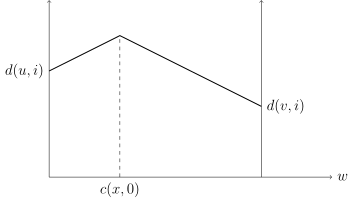
\includegraphics{images/mdst-plot1.png}
	\caption{图的绝对中心变化的影响\cite{oiwiki-dmst}}
	\label{fig:mdst-graph}
\end{figure}

显然可以发现图象会是两条斜率相同的一次函数所构成。

接下来将对于每一个点 $i$ 都画像这样的图象就可以得到:

\begin{figure}[H]
	\centering
	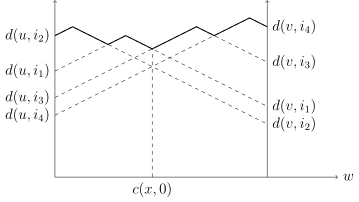
\includegraphics{images/mdst-plot2.png}
	\caption{图的绝对中心变化的影响\cite{oiwiki-dmst}}
	\label{fig:mdst-graph}
\end{figure}

这些折线交点中的最低点,横坐标就是图的绝对中心的位置。

不难发现,出现交点的条件是 $d_{u,i_1} < d_{u,i_2},d_{v,i_1} > d_{v,i_2}$。

对于绝对中心在一个点上,那么就枚举一下那个节点,再用与其距离最远的节点更新一下就行了。

对于每一条边,每一个点都这样做一下就可以了。

总结一下过程:

\begin{enumerate}
    \item 使用最短路算法求出 $d_{i,j}$;
    \item 对于绝对中心在点上更新答案;
    \item 对于绝对中心在边上,枚举每一条边更新答案。
\end{enumerate}

如果使用堆优化的 Dijkstra 求解最短路,时间复杂度为 $\Theta(n^2\log m + nm)$,若使用 Floyd,时间复杂度为 $\Theta(n^3 + nm)$

\subsection{问题二}

\subsubsection{方案一}

可以发现,问题一方案一的结论可以推广到多个核酸检测点。

那只需要枚举两个核酸点,暴力计算取最小值即可。

时间复杂度 $\Theta(n^3)$

\subsubsection{方案二}

\subsection{问题三}

\subsubsection{方案一}

\subsubsection{方案二}

问题转化为给定一张无向图,在其中选择 $k$ 个点,使得每个点距离其最近的核酸检测点距离最大值最小,这个问题不易求解,不妨钦定核酸检测点不会出现在路上(对于一个小区,设置在路上可能会影响交通,所以对最优性影响不大)。

发现问题具有单调性,如果每个点距离最近的核酸检测点距离最大值为 $x$ 的时候可行,那么距离最大值大于等于 $x$ 的时候也可行,这一点是显然的。

那么我们可以进行这样的一个过程,初始时 $l=1,r=n$:

\begin{enumerate}
    \item 判定每个点距离最近的核酸检测点距离最大值 $\frac{l+r}{2}$ 是否可行;
    \item 如若可行,那么可将答案变量设为 $\frac{l+r}{2}$,令 $r = \frac{l+r}{2}-1$;
    \item 如若不可行,令 $l = \frac{l+r}{2} + 1$;
\end{enumerate}

对于一个判定,距离最近的核酸检测点距离最大值为 $x$,我们可以将每个点看成一个集合,第 $i$ 个点所对应的集合 $A_i$ 表示到其距离在 $x$ 以内的点集,那么问题转化为:

给定 $n$ 个集合,第 $i$ 个集合记作 $A_i(\forall j \in A_i, j 
\in [1,n])$,从其中选出 $k$ 个集合构成集合 $\mathscr{A}$,试判断是否存在一种选法,使得 $\bigcup\limits_{S \in \mathscr{A}} S = [1,n]$。

发现这个问题可以被经典 NP-C 问题 SAT 多项式规约,所以它是一个 NP-Hard 问题。

经查证,这是一个经典 NP-Hard 问题,集合覆盖问题(Set cover problem,SCP)\cite{wikipedia-SCP},故精确解只能在非多项式解法中得到,接下来会给出其三种解法,分别为 ILP(整数线性规划),状态压缩动态规划和其近似算法(采用 greedy 算法实现)。

$\textbf{整数线性规划解法}$:

限制:

\begin{equation*}
\begin{cases}
\forall S \in \mathscr{A}, e \in [1,n],\sum_{S;e \in S} x_S \ge 1\\
\forall S \in \mathscr{A}, X_S \in \{0,1\}
\end{cases}
\end{equation*}

然后我们需要最小化 $\sum\limits_{S \in \mathscr{A}} X_S$。

$\textbf{状态压缩动态规划解法}$:

这种做法只能适用于 $n < 20,k \le 10$ 的情况。

假设 $f_{i,S,j}$ 表示前 $i$ 个集合,选了 $j$ 个,并集为 $S$(集中,$S$ 第 $i$ 为 $1$ 表示数字 $i+1$ 已经出现过了)。

设 $A_i$ 对应的 $n$ 位二进制数位 $B_i$。

状态转移:

\begin{equation*}
    f_{i,S,j} = \Big ( \bigvee_{S'\vee B_i = S}{f_{i-1,S',j-1}} \Big ) \vee f_{i-1,S,j}
\end{equation*}

初始状态 $f_{0,0,0} = true$。

时间复杂度 $\Theta(nk2^n)$,空间复杂度 $\Theta(nk2^n)$,空间复杂度可使用滚动数组优化到 $\Theta(2^nk)$。

缺点:只可判断,若需给出解法,空间复杂度变为 $\Theta(4^nk)$,所以最后得到距离最近的核酸检测点距离最大值后还需使用其他方法进行构造解。

$\textbf{近似算法}$:

目前关于集合覆盖问题,仍然找不到一个有效的OPT算法,我们这里提出的是一种基于贪婪策略的近似性算法。

算法过程为如下伪代码:

\begin{algorithm}
    \caption{Greedy Set Cover Algorithm}
    \begin{algorithmic}[1]
        \Require 集合 $A_i$
        \Ensure 选择方式
        \State $C \gets \emptyset$
        \State $\mathscr{A} \gets \emptyset$
        \While{$C \neq [1,n]$}
            \State Find the set $A$ whose $|A\setminus C|$ is biggest
            \State $C = C \cup A$
            \State Add $A$ into $\mathscr{A}$
        \EndWhile
        \State \Return $\mathscr{A}$
    \end{algorithmic}
\end{algorithm}

我们每次选取的都是 $|A\setminus C|$ 最大的集合 $A_i$,即每次新添加的集合 $A$ 的覆盖率都是最大的,从而保证局部最优。

性能分析:

在贪婪算法的每次迭代过程中,剩下元素OPT算法的 $cost$ 必定小于等于原问题OPT算法的 $cost$,即为小于等于 $\frac{|A|}{|[1,n]\setminus C|}$。

设最优解的答案为 $\mathscr{S}$。

接着对于数字 $x$,设 $|C| \le w$,那么显然 $|[1,n]\setminus C| \ge n - w$。

所以数字 $x$ 被覆盖的代价 $\operatorname{price}(x) \le {|A|}{n-w+1}$。

于是就证明了这个近似算法得出的 $|\mathscr{A}| \le H_n \cdot \mathscr{S}$。

所以有 $\sum \operatorname{price}(x) \le (\sum_{i=1}\frac{1}{i}) \cdot \mathscr{S} = H_n \cdot \mathscr{S}$。

不可逼近性结果表明,贪婪算法本质上是集合覆盖到低阶项的最佳多项式时间逼近算法(Dinur&Steurer(2013)通过证明它不能近似于最佳不可近似性来证明最优的不可近似性 ${\displaystyle {\bigl (}1-o(1){\bigr )}\cdot \ln {n}}\text{除非} P{\displaystyle =}NP.)$,在合理的复杂性假设下。对贪婪算法的更严格的分析表明,近似比正好 ${\displaystyle \ln {n}-\ln {\ln {n}}+\Theta(1)}$\cite{greedy-algorithm-for-set-cover}。

对于一个小区,实测答案较为优秀,如下图,我们保证每个点的点权为 $1$(因为这样方便看出优劣),答案为红色的点 $k=10$。

\begin{figure}[H]
	\centering
	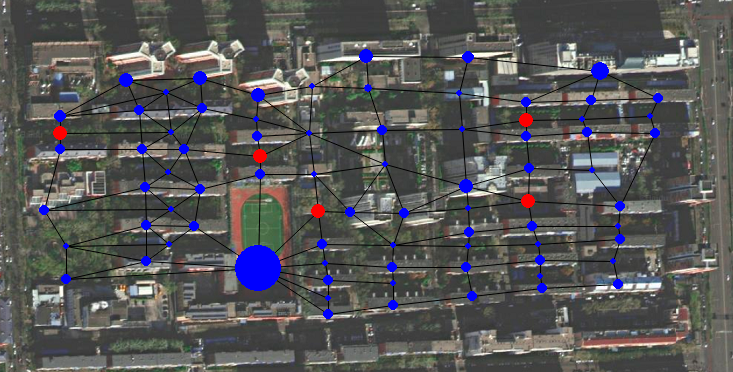
\includegraphics{images/Problem3Subtask2.png}
	\caption{答案}}
	\label{fig:mdst-graph}
\end{figure}

\section{模型评价}

\newpage
\bibliographystyle{plain}
\bibliography{ref}
\newpage

%附录
\begin{appendices}


\section{问题一方案一代码}

\begin{lstlisting}[language=cpp]
#include <iostream>
using namespace std;
typedef long long ll;
const ll INF = 1e18;

int N, M;
ll G[510][510], Dist[510][510], Rank[510][510], W[510];

void Center_Point(int &u, int &v, double &x) { //返回值为绝对中心在边 (u,v),与 u 的距离为 x
    for (int k = 1; k <= N; k++) {
        for (int i = 1; i <= N; i++) {
            for (int j = 1; j <= N; j++) {
                Dist[i][j] = min(Dist[i][j], Dist[i][k] + Dist[k][j]);
            }
        }
    }

    for (int i = 1; i <= N; i++) {
        for (int j = 1; j <= N; j++) Rank[i][j] = j;
        for (int j = 1; j <= N; j++) {
            for (int k = j + 1; k <= N; k++) {
                if (Dist[i][Rank[i][j]] > Dist[i][Rank[i][k]]) {
                    swap(Dist[i][Rank[i][j]], Dist[i][Rank[i][k]]);
                }
            }
        }
    }

    double Ans = 1e18;

    for (int i = 1; i <= N; i++) {
        for (int j = 1; j <= N; j++) {
            if (i == j || G[i][j] == INF) continue;
            int p = Rank[i][N];
            ll Temp = W[i] * Dist[i][p];
            if (Ans > Temp) {
                Ans = Temp;
                u = i;
                v = j;
                x = 0.00;
            }
            for (int k = N - 1; k >= 1; k--) {
                int t = Rank[i][k];
                if (Dist[j][t] > Dist[j][p]) {
                    Temp = W[i] * (Dist[i][t] + Dist[j][p] + G[i][j]);
                    if (Ans > Temp) {
                        Ans = Temp;
                        u = i;
                        v = j;
                        x = (Dist[j][p] + Dist[i][j] - Dist[i][t]) / 2.00;
                    }
                    p = t;
                }
            }
        }
    }
    return;
}
\end{lstlisting}

\section{问题一方案二代码}

\begin{lstlisting}[language=cpp]
#include <iostream>
using namespace std;
typedef long long ll;
const ll INF = 1e18;

int N, M;
ll G[510][510], Dist[510][510], Rank[510][510], W[510];

int Solve() { // 返回核酸检测点位置
    for (int k = 1; k <= N; k++) {
        for (int i = 1; i <= N; i++) {
            for (int j = 1; j <= N; j++) {
                Dist[i][j] = min(Dist[i][j], Dist[i][k] + Dist[k][j]);
            }
        }
    }

    int ans=0;ll r=INF;
    for(int i = 1; i <= N; i++){
        ll t=0;
        for(int j = 1;j <= N; j++){
            t += Dist[i][j] * W[j];
        }
        if(t<r) ans = i, r = t;
    }

    return ans;
    
    return;
}
\end{lstlisting}

\section{问题三方案二代码}

\begin{lstlisting}
#include <bits/stdc++.h>
using namespace std;
const int MAXN = 510;

int N, M, K;
bitset<MAXN> A[MAXN], U;
long long W[MAXN];
long long G[MAXN][MAXN];
bitset<MAXN> Ans;

bool Check(long long x) {
    vector<int> S;
    bitset<MAXN> C;
    for (int i = 1; i <= N; i++) A[i].reset();
    for (int i = 1; i <= N; i++) {
        for (int j = 1; j <= N; j++) {
            if (W[i] * G[i][j] <= x) {
                A[i][j] = true;
            }
        }
    }
    while (C != U) {
        pair<int, int> Max = {0, 0};
        for (int i = 1; i <= N; i++) {
            int x = 0;
            for (int j = 1; j <= N; j++) {
                if (A[i][j] == 1 && C[j] == 0) {
                    x++;
                }
            }
            if (x > Max.first) {
                Max = {x, i};
            }
        }
        C = C | A[Max.second];
        S.push_back(Max.second);
        if (S.size() > K) return false;
    }
    Ans.reset();
    for (int i : S) Ans[i] = true;
    return true;
}

int main() {
    scanf("%d %d %d" ,&N ,&M ,&K);
    memset(G, 0x3f, sizeof G);
    for (int i = 1; i <= N; i++) {
        scanf("%d" ,&W[i]);
        W[i]++;
        G[i][i] = 0;
        U[i] = true;
    }
    for (int i = 1; i <= M; i++) {
        static int u, v, w;
        scanf("%d %d %d" ,&u ,&v ,&w);
        G[u][v] = w;
        G[v][u] = w;
    }
    for (int k = 1; k <= N; k++) {
        for (int i = 1; i <= N; i++) {
            for (int j = 1; j <= N; j++) {
                G[i][j] = min(G[i][k] + G[k][j], G[i][j]);
            }
        }
    }
    long long l = 1, r = 0;
    for (int i = 1; i <= N; i++) {
        for (int j = 1; j <= N; j++) {
            r = max(r, W[i] * G[i][j]);
        }
    }
    while (l <= r) {
        long long mid = l + r >> 1;
        if (Check(mid)) r = mid - 1;
        else l = mid + 1; 
    }
    for (int i = 1; i <= N; i++) {
        if (Ans[i]) {
            cout << i << " ";
        }
    }
    return 0;
}
\end{lstlisting}

\end{appendices}

\end{document} 